\documentclass[xcolor=svgnames]{beamer}
\usepackage{graphics}
\usepackage{amsmath}
\usepackage[english]{babel}
\usetheme{Warsaw}
\useinnertheme{rounded}
\usefonttheme{serif}
\setbeamertemplate{navigation symbols}{}
\begin{document}
\title{M311 Calculus III Recitation}
	\author{Tim Lai }
	\institute{Indiana University}
%	\titlegraphic{\includegraphics[width=5cm]{Logo.jpg}}
	\date{Fall 2019}
\frame{\titlepage}
\begin{frame}
\frametitle{Projections}
\framesubtitle{Section 12.1}
\begin{center}
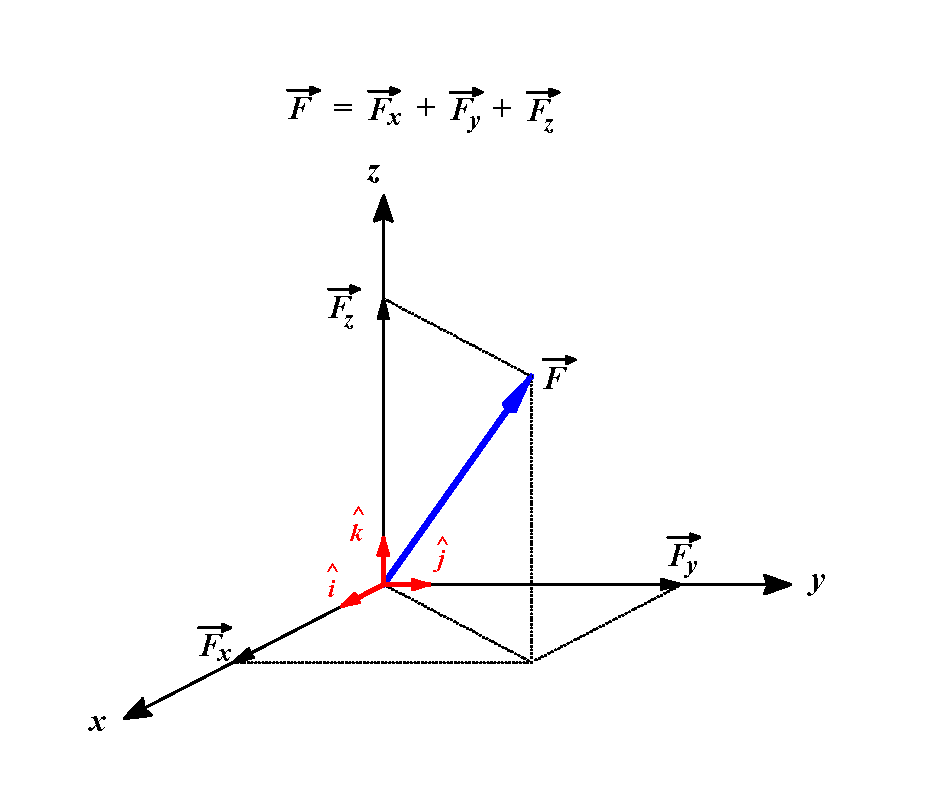
\includegraphics[width=8cm]{3D_vector_component.png}
\end{center}
\end{frame}
\begin{frame}
\frametitle{Vector Operations}
\framesubtitle{Section 12.2}
Suppose $a = \langle 2,3,0 \rangle$ and $b = \langle -1, 0,1 \rangle$. 
Then
\begin{align*}
 |a + 2b| &= |  \langle 2,3,0 \rangle + 2  \langle -1, 0,1 \rangle | \\
&= | \langle 2,3,0 \rangle +\langle -2, 0,2 \rangle | \\
& = | \langle 0,3,2 \rangle | \\
&= \sqrt{0^2 + 3^2 + 2^2} \\
&= \sqrt{13}
\end{align*}
\end{frame}
\begin{frame}
\frametitle{Dot Product}
\framesubtitle{Section 12.3}
Dot products are a special case of matrix multiplication.

Suppose $a = \langle 2,3,0 \rangle$ and $b = \langle -1, 0,1 \rangle$. Then
\[
 a \cdot b = 2(-1) + 3(0) + 0(1) = -2
\]
Compare to $(2,3,0) (-1,0,1)^T$ where these are now thought of as matrices and $T$ denotes transpose. 
\end{frame}
\begin{frame}
\frametitle{Dot Product}
\framesubtitle{Important properties and uses}
\begin{itemize}
	\item Dot product gives a computationally conducive way to get a handle on angles between vectors. 
	\item $a \cdot b = |a||b| \cos \theta$ where $\theta$ is the angle between the two vectors. 
	\item In particular, since $\cos \theta = 0$ if and only if $\theta = \pi / 2 + k \pi$, we can conclude that $a \perp b \Leftrightarrow a \cdot b = 0$. 
	\item Note: dot product takes two vectors and gives a number. 
	\item In the previous example, since the dot product was nonzero, we can conclusively say that the vectors were not orthogonal. 
\end{itemize}
\end{frame}


\end{document}